%Chapter 7

\chapter{On the Transferability of Deep-Q Networks} % Chapter title
\label{ch:dqn_transfer} % For referencing the chapter elsewhere, use \autoref{ch:introduction} 

\begin{remark}{Outline}
\end{remark}


\section{Motivation}


\section{A large-scale Empirical Study}

\subsection{Experimental Setup}

\subsection{Results}


\section{Control Experiments}

\subsection{Catcher Environments}
\begin{figure}%
    \centering
    \subfloat[\centering label 1]{{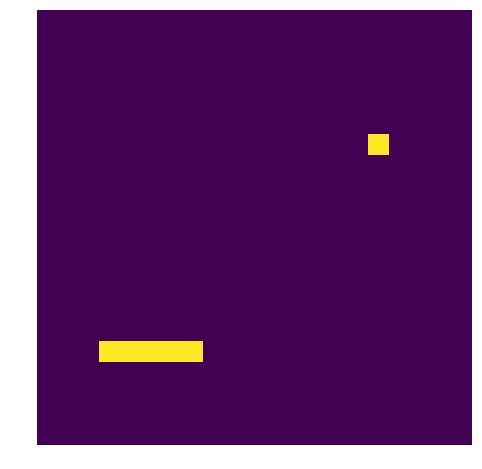
\includegraphics[width=3cm]{./Images/Chapter08/catch_v0} }}%
    \qquad
    \subfloat[\centering label 2]{{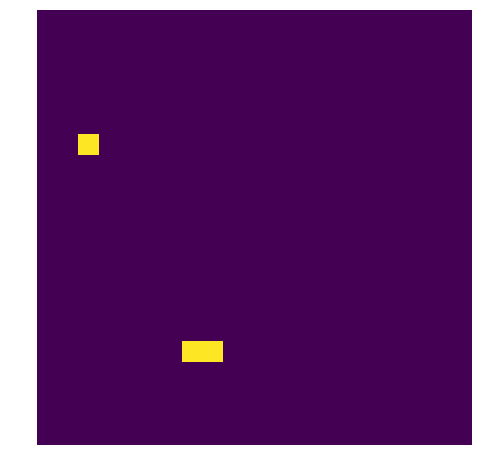
\includegraphics[width=3cm]{./Images/Chapter08/catch_v2} }}%
     \qquad
    \subfloat[\centering label 3]{{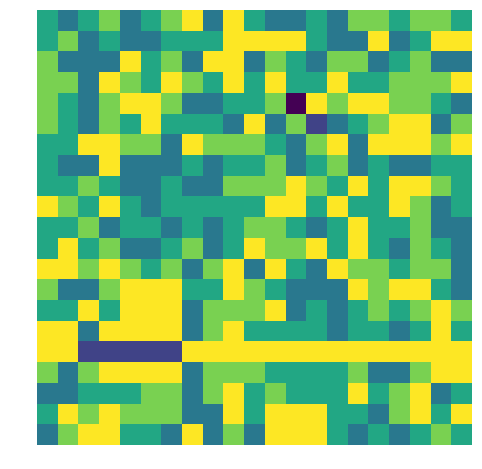
\includegraphics[width=3cm]{./Images/Chapter08/catch_v3} }}%
     \qquad
    \subfloat[\centering label 4]{{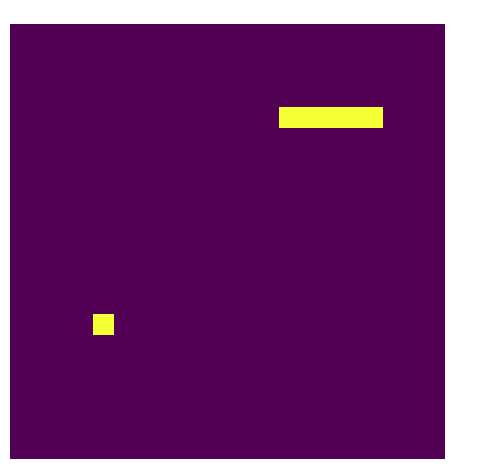
\includegraphics[width=3cm]{./Images/Chapter08/catch_v1} }}% 
    \caption{2 Figures side by side}%
    \label{fig:example}%
\end{figure}


\subsection{From one Catcher to Another}

\subsection{Self-Transfer}
